\documentclass[a4paper,12pt]{article}
\usepackage[a4paper,top=1.3cm,bottom=2cm,left=1.5cm,right=1.5cm,marginparwidth=0.75cm]{geometry}
\usepackage{cmap}
\usepackage{mathtext}
\usepackage[T2A]{fontenc}
\usepackage[utf8]{inputenc}
\usepackage[english,russian]{babel}
\usepackage{siunitx}
\usepackage{enumitem}
\usepackage{placeins}

\usepackage{graphicx}

\usepackage{wrapfig}
\usepackage{tabularx}
\usepackage{multirow}

\usepackage{hyperref}
\usepackage[rgb]{xcolor}
\hypersetup{
colorlinks=true,urlcolor=blue
}
\usepackage{amsmath,amsfonts,amssymb,amsthm,mathtools}
\usepackage{icomma}
\mathtoolsset{showonlyrefs=false}
\usepackage{euscript}
\usepackage{mathrsfs}
\DeclareMathOperator{\sgn}{\mathop{sgn}}
\newcommand*{\hm}[1]{#1\nobreak\discretionary{}
{\hbox{$\mathsurround=0pt #1$}}{}}

%%% Заголовок
\author{Макаров Лев Евгеньевич}
\title{Лабораторная работа №3.2.5

Свободные и вынужденные колебания в электрическом контуре
}
\date{\today}

\begin{document}

\begin{titlepage}
	\begin{center}
		{\large МОСКОВСКИЙ ФИЗИКО-ТЕХНИЧЕСКИЙ ИНСТИТУТ (НАЦИОНАЛЬНЫЙ ИССЛЕДОВАТЕЛЬСКИЙ УНИВЕРСИТЕТ)}
	\end{center}
	\begin{center}
		{\large Физтех-школа фотоники, электроники и молекулярной физики}
	\end{center}
	
	
	\vspace{4.5cm}
	{\huge
		\begin{center}
			{\bf Отчёт о выполнении лабораторной работы 3.2.5}\\
			Свободные и вынужденные колебания в электрическом контуре
		\end{center}
	}
	\vspace{2cm}
	\begin{flushright}
		{\LARGE Автор:\\ Макаров Лев Евгеньевич \\
			\vspace{0.2cm}
			Б04-306}
	\end{flushright}
	\vspace{8cm}
	\begin{center}
		Долгопрудный 2024
	\end{center}
\end{titlepage}


\textbf{Цель работы:} 
\begin{enumerate}
	\item исследование свободных и вынужденных колебаний в колебательном контуре
\end{enumerate}

\textbf{В работе используются:} 
\begin{itemize}
    \item осциллограф АКТАКОМ ADS-6142H
    \item генератор сигналов специальной формы АКИП-3409/4
    \item магазин сопротивления МСР-60
    \item магазин емкости Р5025
    \item магазин индуктивности Р567 типа МИСП
    \item соединительная коробка с шунтирующей емкостью
    \item соединительные одножильные и коаксиальные провода
\end{itemize}
\medskip

\section{Экспериментальная установка}

Схема установки для исследования колебаний приведена на рисунке \ref{pic:1}.

Колебательный контур состоит из постоянной индуктивности $L$ с активным сопротивлением $R_L$, переменной емкости $C$ и сопротивления $R$. Картина колебаний напряжения на емкости наблюдается на экране двухканального осциллографа. Для возбуждения затухающих колебаний используется генератор сигналов специальной формы. Сигнал с генератора поступает через конденсатор $C_1$ на вход колебательного контура. Данная емкость необходима чтобы выходной импеданс генератора был много меньше импеданса колебательного контура и не влиял на процессы, проходящие в контуре.

\begin{figure}[h!]
    \includegraphics[width=0.8\textwidth]{ust_1.png}
    \caption{\textit{Схема установки для исследования вынужденных колебаний}}
    \label{pic:1}
\end{figure}

Установка предназначена для исследования не только возбужденных, но и свободных колебаний в электрической цепи. При изучении свободно затухающих колебаний генератор специальных сигналов на вход колебательного контура подает периодические короткие импульсы, которые заряжают конденсатор $C$. За время между последовательными импульсами происходит разрядка конденсатора через резистор и катушку индуктивности. Напряжение на конденсаторе $U_C$ поступает на вход канала $1(X)$ электронного осциллографа. Для наблюдения фазовой картины затухающих колебаний на канал $2(Y)$ подается напряжение с резистора $R$ (пунктирная линия на схеме установки), которое пропорционально току $I (I \propto d U_C / dt)$.

При изучении возбужденных колебаний на вход колебательного контура подается синусоидальный сигнал. С помощью осциллографа возможно измерить зависимость амплитуды возбужденных колебаний в зависимости от частоты внешнего сигнала, из которого возможно определить добротность колебательного контура. Альтернативным способом расчета добротности контура является определение декремента затухания по картине установления возбужденных колебаний. В этом случае генератор сигналов используется для подачи цугов синусоидальной формы.

\section{Результаты измерений и обработка данных}

\subsection{Подготовка приборов к работе}

\begin{enumerate}
    \item Подключим генератор ко входу $1(X)$
    \item Установим на генераторе режим "Pulse" с длительностью импульсов 10 мкс, частотой повторения 100 Гц и амплитудой 20 В.
    \item Убедимся, что на осциллограф поступает нужный сигнал. Нажмем "Autoset" и выставим нужный уровень "Trigger".
    \item Соберем схему согласно рис. \ref{pic:1}
\end{enumerate}

\subsection{Измерение периодов свободных колебаний}

\begin{enumerate}
    \item Установим сопротивление $R = 0$ Ом, индуктивность $L = 100$ мГ, емкость $C = 0$ мкФ. Определим минимальную емкость магазина емкостей $C_0$. Получим картину затухающих колебаний в контуре.
    \item Подберем частоту развертки так, чтобы расстояние между импульсами занимало почти весь экран.
    \item Измерим период затухающих колебаний с помощью осциллографа
\end{enumerate}

Нажмем "Cursor", выберем время и выставим линии-указатели на два соседних максимума

\begin{equation*}
    T_0 = 55 \ \text{мкс}
\end{equation*}

\begin{enumerate}[resume]
    \item Вычислим $C_0$
\end{enumerate}

\begin{equation*}
    T = 2 \pi \sqrt{L C_0} \implies C_0 = \frac{T_0^2}{4 \pi^2 L} \approx 0,77 \ \text{нФ}
\end{equation*}

\begin{enumerate}[resume]
    \item Повторим измерения для еще 9 значение $C$. Результаты измерений запишем в таблицу \ref{table:1}.
\end{enumerate}

\begin{table}[!ht!]
    \centering
    \begin{tabular}{|l|l|l|}
    \hline
        $C$, нФ & $C + C_0$, нФ & $\Delta x$, мс \\ \hline
        0 & 0,77 & 0,055 \\ \hline
        1 & 1,77 & 0,0736 \\ \hline
        2 & 2,77 & 0,0884 \\ \hline
        3 & 3,77 & 0,101 \\ \hline
        4 & 4,77 & 0,113 \\ \hline
        5 & 5,77 & 0,122 \\ \hline
        6 & 6,77 & 0,132 \\ \hline
        7 & 7,77 & 0,143 \\ \hline
        8 & 8,77 & 0,149 \\ \hline
        9 & 9,77 & 0,159 \\ \hline
    \end{tabular}\caption{\textit{Измерение периода колебаний от емкости}}\label{table:1}
\end{table}

\FloatBarrier

\subsection{Критическое сопротивление и декремент затухания}

\begin{enumerate}
    \item Рассчитаем $C^*$, при которой $\nu_0 = 6,5$ кГц
\end{enumerate}

\begin{equation*}
    \nu_0 = \frac{1}{2 \pi \sqrt{L C^*}} \implies C^* = \frac{1}{4 \pi^2 \nu_0^2 L} \approx 6 \ \text{нФ}
\end{equation*}

Для $C^*$ и $L$ рассчитаем критическое сопротивление контура $R_{cr}$

\begin{equation*}
    R_{cr} = 2 \sqrt{\frac{L}{C^*}} \approx 8168 \ \text{Ом}
\end{equation*}

\begin{enumerate}[resume]
    \item Установим $R$ близкое к $R_{cr}$ и наблюдаем, что затухающие колебания при изменении от $0$ до $R_{cr}$ переходит в апериодический режим.
    \item Установим сопротивление $R = 0,05 R_cr \approx 408,4 \text{Ом}$. Вычислим логарифмический декремент затухания.
\end{enumerate}

Замерим разницу амплитуд между максимумами для сопротивления и результаты измерений запишем в таблицу \ref{table:2}.

\begin{enumerate}[resume]
    \item Повторим результаты измерений прошлого пункта для значений $R$ от $0,05 R_{cr}$ до $0,25 R_{cr}$. Результаты измерений запишем в таблицу \ref{table:2}
\end{enumerate}

\begin{table}[!ht]
    \centering
    \begin{tabular}{|l|l|l|l|l|l|l|}
    \hline
        $N$ & $R$, Ом & $U_m$, мВ & $U_{m+n}$, мВ & $m$ & $n$ & $\theta$ \\ \hline
        1 & 408,4 & 1300 & 320 & 1 & 4 & 0,35 \\ \hline
        2 & 680,6 & 1060 & 240 & 1 & 3 & 0,50 \\ \hline
        3 & 952,9 & 920 & 140 & 1 & 3 & 0,63 \\ \hline
        4 & 1225,2 & 776 & 64 & 1 & 3 & 0,83 \\ \hline
        5 & 1497,5 & 680 & 80 & 1 & 2 & 1,07 \\ \hline
        6 & 1769,7 & 568 & 72 & 1 & 2 & 1,03 \\ \hline
        7 & 2042,0 & 496 & 104 & 1 & 1 & 1,56 \\ \hline
    \end{tabular}\caption{\textit{Измерение периода колебаний от емкости}}\label{table:2}
\end{table}

\FloatBarrier

\begin{enumerate}[resume]
    \item Зафиксируем значения сопротивления $R_1 = 408,4$ Ом и $R_2 = 2042,0$ Ом.
\end{enumerate}

\subsection{Свободные колебания на фазовой плоскости}

\begin{enumerate}
    \item Выставим сопротивление $R_1$ на магазине. Подадим на канал $2(Y)$ падение напряжения с резистора
    \item Переведем осциллограф в двухканальный режим. Подберем масштабы так, чтобы можно было наблюдать оба сигнала.
    \item Подберем частоту так, чтобы расстояние между импульса примерно совпадала со временем затухания колебаний.
\end{enumerate}

\begin{equation*}
    \nu = 470 \ \text{Гц}
\end{equation*}

\begin{enumerate}[resume]
    \item Пронаблюдаем фазовые колебания в плоскости. Для этого выберем режим XY через кнопку "Display".
\end{enumerate}

Понаблюдать спираль получилось только для одного сопротивления $R = R_1$. Для него посчитаем логарифмический декремент затухания:

\begin{equation*}
    \theta = \frac{1}{n} \ln{\frac{N_m}{N_{n+m}}} = \frac{1}{1} \ln {\frac{17}{11}} \approx 0,44
\end{equation*}

\subsection{Исследование резонансных кривых}

\begin{enumerate}
    \item Переведем осциллограф в одноканальный режим просмотра
    \item Переведем генератор в режим подачи синусоидальных сигналов
    \item Выставим емкость $C = C^*$ и сопротивление $R = R_1$
    \item Модифицируем схему согласно рис. \ref{pic:2}. Добьемся того, чтобы можно было одновременно наблюдать оба сигнала на осциллографе.
\end{enumerate}

\begin{figure}[h!]
    \includegraphics[width=0.8\textwidth]{ust_2.png}
    \caption{\textit{Схема установки для исследования АЧХ и ФЧХ}}
    \label{pic:2}
\end{figure}

\FloatBarrier

\begin{enumerate}[resume]
    \item Убедимся, что вблизи резонансной частоты -- устойчивый синусоидальный сигнал
    \item Убедимся, что вблизи резонансной частоты амплитуда колебаний максимальна именно при резонансной частоте. Определим ее значение
    \item Снимем АЧХ и ФЧХ колебательного контура
\end{enumerate}

Настроим генератор на резонансную частоту, определим амплитуду $U_{res} = 8,88$ В.определим диапазон частот, в которых амплитуда не меньше $0,4 \cdot U_{res}$. Проведем по 10 измерений амплитуды от частоты при смещении частоты в каждую сторону от резонансной. Результаты измерений запишем в таблицу \ref{table:3}.

\begin{table}[!ht]
    \centering
    \begin{tabular}{|l|l|l|l|}
    \hline
        $N$ & $\nu$, кГц & $U_{R1}$, В & $U_{R2}$ \\ \hline
        0 & 5,26 & 3,56 & 1,89 \\ \hline
        1 & 5,35 & 4,06 & 1,95 \\ \hline
        2 & 5,44 & 4,76 & 2,03 \\ \hline
        3 & 5,53 & 5,46 & 2,08 \\ \hline
        4 & 5,62 & 6,26 & 2,15 \\ \hline
        5 & 5,71 & 7,26 & 2,20 \\ \hline
        6 & 5,80 & 8,12 & 2,26 \\ \hline
        7 & 5,89 & 8,74 & 2,30 \\ \hline
        8 & 5,98 & 8,92 & 2,33 \\ \hline
        9 & 6,07 & 8,66 & 2,33 \\ \hline
        10 & 6,16 & 8,06 & 2,35 \\ \hline
        11 & 6,25 & 7,38 & 2,31 \\ \hline
        12 & 6,34 & 6,60 & 2,31 \\ \hline
        13 & 6,43 & 6,00 & 2,31 \\ \hline
        14 & 6,52 & 5,50 & 2,32 \\ \hline
        15 & 6,61 & 5,08 & 2,34 \\ \hline
        16 & 6,70 & 4,62 & 2,34 \\ \hline
        17 & 6,79 & 4,28 & 2,31 \\ \hline
        18 & 6,88 & 4,02 & 2,30 \\ \hline
        19 & 6,97 & 3,82 & 2,26 \\ \hline
    \end{tabular}\caption{\textit{Измерение АЧХ и ФЧХ колебательного контура}}\label{table:3}
\end{table}

\begin{enumerate}[resume]
    \item Повторим измерения предыдущего пункта для $R = R_2$, результаты запишем в таблицу \ref{table:3}.
\end{enumerate}

\subsection{Процессы установления и затухания}

\begin{enumerate}
    \item Установим сопротивление $R = R_1$
    \item Установим резонансную частоту на генераторе
    \item Включим режим "Burst" на генераторе
    \item Установим период повторения 20 мс, и количевство периодов 15
    \item Получим характерную картину колебаний для одного цуга.
    \item Для определения добротности по скорости нарастания измерим амплитуды колебаний, разделенных целым числом периодов и амплитуду установившихся колебаний. Результаты измерений запишем в таблицу \ref{table:4}
\end{enumerate}

\begin{table}[!ht]
    \centering
    \begin{tabular}{|l|l|l|l|l|l|}
    \hline
        $U_0$, В & $U_k$, В & $U_{k + n}$, В & $k$ & $n$ & $\theta$ \\ \hline
        8,88 & 5,24 & 7,26 & 3 & 2 & 0,40 \\ \hline
        8,88 & 5,24 & 6,44 & 3 & 1 & 0,40 \\ \hline
        8,88 & 5,24 & 8,4 & 3 & 5 & 0,41 \\ \hline
    \end{tabular}\caption{\textit{Измерение добротности по скорости нарастания колебаний}}\label{table:4}
\end{table}

\FloatBarrier

\begin{enumerate}[resume]
    \item Посчитаем логарифмический декремент нарастания по формуле (запишем в таблицу \ref{table:4})
\end{enumerate}

\begin{equation*}
    \theta = \frac{1}{n} \ln{\frac{U_0 - U_k}{U_0 - U_{k + n}}}
\end{equation*}

\begin{enumerate}[resume]
    \item Для определения добротности по скорости затухания измерим амплитуды колебаний, разделенных целым числом периодов и амплитуду установившихся колебаний. Результаты измерений запишем в таблицу \ref{table:5}
\end{enumerate}

\begin{table}[!ht]
    \centering
    \begin{tabular}{|l|l|l|l|l|}
    \hline
        $U_k$, В & $U_{k + n}$, В & $k$ & $n$ & $\theta$ \\ \hline
        8,72 & 5,92 & 1 & 1 & 0,39 \\ \hline
        8,72 & 4,04 & 1 & 2 & 0,38 \\ \hline
        8,72 & 2,76 & 1 & 3 & 0,38 \\ \hline
    \end{tabular}\caption{\textit{Измерение добротности по скорости нарастания колебаний}}\label{table:5}
\end{table}

\begin{enumerate}[resume]
    \item Посчитаем логарифмический декремент затухания и запишем в таблицу \ref{table:5}
    \item Повторим измерения предыдущих пунктов для сопротивления $R = R_2$. Результаты измерений запишем в таблицы \ref{table:6} и \ref{table:7}
\end{enumerate}

\begin{table}[!ht]
    \centering
    \begin{tabular}{|l|l|l|l|l|l|}
    \hline
        $U_0$, В & $U_k$, В & $U_{k + n}$, В & $k$ & $n$ & $\theta$ \\ \hline
        2,4 & 2 & 0,84 & 3 & 1 & 1,36 \\ \hline
    \end{tabular}\caption{\textit{Измерение добротности по скорости нарастания колебаний для $R_2$}}\label{table:6}
\end{table}

\begin{table}[!ht]
    \centering
    \begin{tabular}{|l|l|l|l|l|}
    \hline
        $U_k$, В & $U_{k + n}$, В & $k$ & $n$ & $\theta$ \\ \hline
        1,96 & 0,4 & 1 & 1 & 1,6 \\ \hline
    \end{tabular}\caption{\textit{Измерение добротности по скорости нарастания колебаний для $R_2$}}\label{table:7}
\end{table}

\begin{enumerate}[resume]
    \item Вернем сопротивление $R_1$. Сместим частоту генератора и получим картину биений.
\end{enumerate}

Картина биений получается из-за того, что разница частот генератора и колебательной системы мала по сравнению с характерным временем установления постоянного режима вынужденных колебаний, через некоторое время после установления произойдёт затухание амплитуды колебаний, связанное с нарастающей разностью фаз между генератором и системой.

\begin{enumerate}[resume]
    \item Отключим все приборы от сети
    \item Измерим активное сопротивление $R_L$ и индуктивность $L$ магазина индуктивностей
\end{enumerate}

\begin{table}[]
    \centering
    \begin{tabular}{|l|l|l|}
    \hline
        $\nu$, Гц & $R_L$, Ом & $L$, мГн \\ \hline
        50 & 23,168 & 99,958 \\ \hline
        500 & 23,243 & 99,921 \\ \hline
        1500 & 24,609 & 99,961 \\ \hline
    \end{tabular}
    \caption{\textit{Измерение $R_L$ и $L$}}\label{table:7}
\end{table}

\FloatBarrier

\subsection{Обработка результатов}

\begin{enumerate}
    \item Рассчитаем экспериментальное значение периодов и теоретические. Построим график зависимости $T_{exp} = f(T_{theor})$. График изобразим на рисунке \ref{graph:1}
\end{enumerate}


\begin{figure}[!ht]
        \centering
	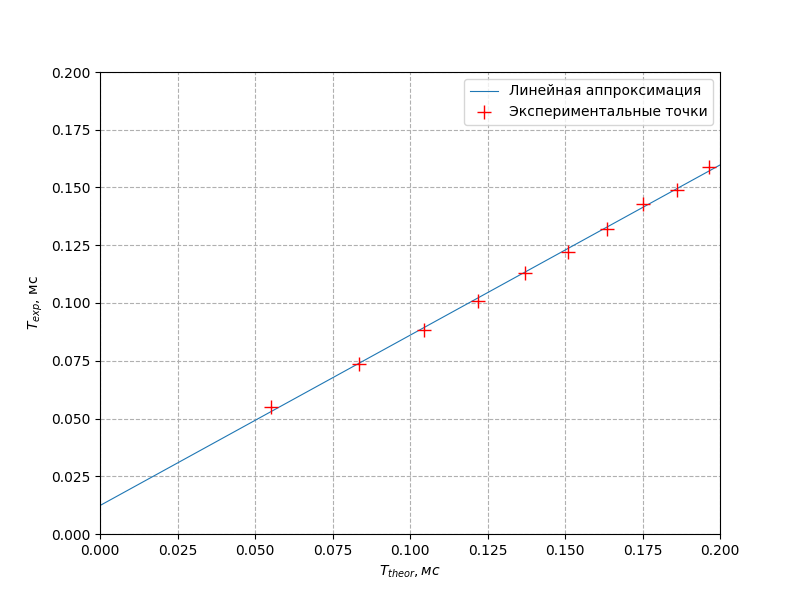
\includegraphics[width=1.0\textwidth]{graph-1.png}
	\caption{\textit{Зависимость $T_{exp} = f(T_{theor})$}}
	\label{graph:1}
\end{figure}

В данном случае зависимость -- линейная, аппроксимируется прямой с параметрами:

\begin{equation*}
    k = (0,737 \pm 0,009) \ \ \ \ \ b = (0,0123 \pm 0,0004) \ \text{мс}
\end{equation*}

\FloatBarrier

\begin{enumerate}[resume]
    \item Рассчитаем значение логарифмического декремента затухания $\theta$ и сопротивление контура $R_\Sigma$.
\end{enumerate}

Построим график в координатах $1/ \theta^2 = f \left( 1/R_\Sigma^2 \right)$. График изобразим на рисунке \ref{graph:2}


\begin{figure}[!ht]
        \centering
	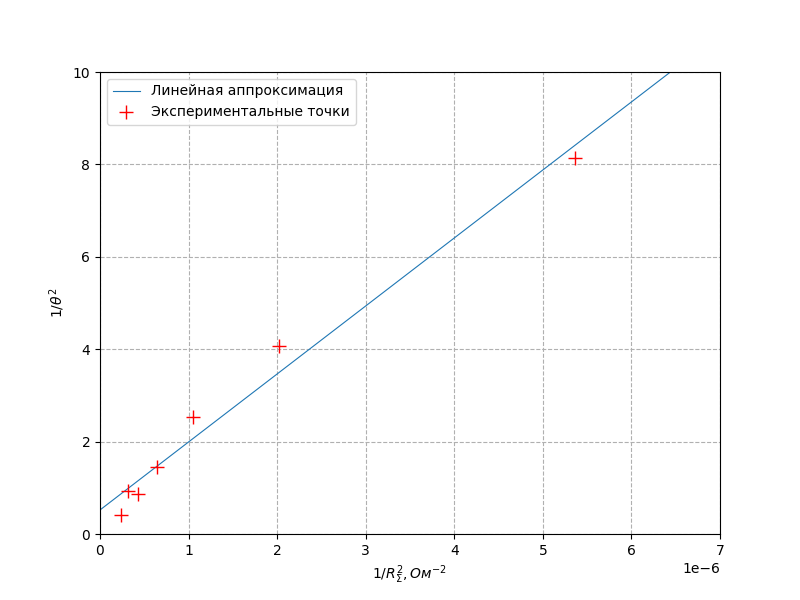
\includegraphics[width=1.0\textwidth]{graph-2.png}
	\caption{\textit{Зависимость $1/ \theta^2 = f \left( 1/R_\Sigma^2 \right)$}}
	\label{graph:2}
\end{figure}

\FloatBarrier

Параметры прямой 

\begin{equation*}
    k = (1470000 \pm 80000) \ \text{Ом}^2 \ \ \ \ \ b = (0,5 \pm 0,1)
\end{equation*}

Наклон графика вблизи начала координат:

\begin{equation*}
    \frac{\Delta Y}{\Delta X} = (2343255 \pm 1) \ \text{Ом}^2
\end{equation*}

Тогда 

\begin{equation*}
    R_{cr} = 2 \pi \sqrt{\frac{\Delta Y}{\Delta X}} = (9618,108 \pm 0,004) \ \text{Ом}
\end{equation*}

\begin{enumerate}[resume]
    \item Теоретическое значение $R_{cr} = 8168$ Ом. Как видно значения не совпали в пределах погрешности.
    \item рассчитаем добротность контура
\end{enumerate}

\begin{equation*}
    Q_1 = \frac{\pi}{\theta^{min}} \approx 10
\end{equation*}
\begin{equation*}
    Q_2 = \frac{\pi}{\theta^{max}} \approx 2
\end{equation*}

\begin{enumerate}[resume]
    \item Добротность по спирали на фазовой плосксти $Q = 7$
    \item Теоретическое значение добротности
\end{enumerate}

\begin{equation*}
    Q^{theor} = \frac{\pi}{\theta} = \frac{\pi}{\gamma T} = \frac{\pi}{\frac{R}{2L}\frac{2\pi}{\omega_1}} = \frac{L}{R}\omega_1 = \frac{L}{R}\sqrt{\omega_0^2 - \gamma^2} = \frac{L}{R}\sqrt{\frac{1}{LC} - \frac{R^2}{4L^2}} = \frac{1}{2}\sqrt{\frac{4L}{CR^2} - 1}
\end{equation*}

\begin{equation*}
    Q_1^{theor} \approx 10
\end{equation*}
\begin{equation*}
    Q_2^{theor} \approx 2
\end{equation*}

Как видимо теоретическое значение хорошо совпало с экспериментальным

\begin{enumerate}[resume]
    \item Построим на одном графике резонансные кривые $U/U_0 = f(\nu/\nu_0)$
\end{enumerate}

\begin{figure}[!ht]
        \centering
	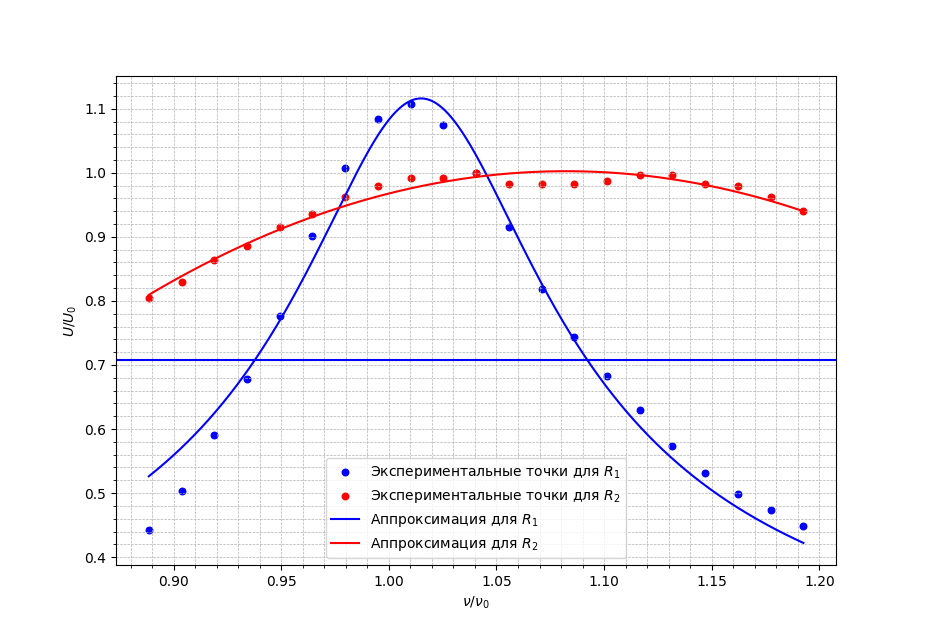
\includegraphics[width=1.0\textwidth]{graph-3.png}
	\caption{\textit{АЧХ}}
	\label{graph:3}
\end{figure}

\begin{enumerate}[resume]
    \item Измерим добротность по ширине резонансной кривой на уровне $1/ \sqrt{2}$
\end{enumerate}

\begin{equation*}
    Q_1 = \frac{\omega_0}{2 \Delta \Omega} \approx 3
\end{equation*}

\begin{enumerate}[resume]
    \item Добротность по ФЧХ
\end{enumerate}

Добротность по ФЧХ вычисляется:

\begin{equation*}
    Q = \frac{\omega_0}{\Delta \omega}
\end{equation*}

\begin{enumerate}[resume]
    \item Построим ФЧХ для $R_1$ и $R_2$ на одном графике
\end{enumerate}




\end{document}